\documentclass[10pt,twocolumn,letterpaper]{article}

\usepackage{cvpr}
%\usepackage{times}
\usepackage{epsfig}
\usepackage{graphicx}
\usepackage{amsmath}
\usepackage{amssymb}

% Include other packages here, before hyperref.

% If you comment hyperref and then uncomment it, you should delete
% egpaper.aux before re-running latex.  (Or just hit 'q' on the first latex
% run, let it finish, and you should be clear).
\usepackage[breaklinks=true,bookmarks=false]{hyperref}

\cvprfinalcopy % *** Uncomment this line for the final submission

\def\cvprPaperID{****} % *** Enter the CVPR Paper ID here
\def\httilde{\mbox{\tt\raisebox{-.5ex}{\symbol{126}}}}

% Pages are numbered in submission mode, and unnumbered in camera-ready
%\ifcvprfinal\pagestyle{empty}\fi
\setcounter{page}{1}
\begin{document}

%-------------------------------------------------------------------------
\title{Deep Learning for 3D Brain Activity Scans}

\author{Anonymized for Peer Review\\
University of Massachusetts Amherst\\
140 Governors Dr, Amherst, MA 01002\\
{\tt\small @umass.edu}
}

\maketitle
%\thispagestyle{empty}

% ------------------------------------------------------------------------
% ABSTRACT
%-------------------------------------------------------------------------
\begin{abstract}
 Analyzing the brain's activity patterns starts with identifying known patterns of well established structures,
 typically observed by human oversight in two dimensions, which may miss subtle, barely visible but useful indicators,
 and limit the ability to stitch together patterns across a third dimension.

 Deep learning's ability to decipher and learn from such nearly impossible patterns in massive datasets,
 imperceptible to preliminary observation makes it an excellent candidate to explore and teach us about
 overlooked patterns of activity.

 Here I showcase convolutional network's ability to correctly classify uncleaned activity data from a passive
 image viewing experiment aimed at triggering activity in particular regions of the brain controlling reward and
 restraint, using the data in both 2d and 3d to explore the merits of adapting video-processing techniques meant
 to apply across time to a third spatial dimension and discuss adapting this to unsupervised segmentation to see
 what the network can teach us from its findings.

\end{abstract}

% ------------------------------------------------------------------------
% BODY
%-------------------------------------------------------------------------
\section{Introduction}\label{sec:introduction}

Neuroimaging presents fertile grounds for deep learning applications, with myriad interesting real world benefits
for mental health research and disease diagnosis.
High dimensional, massive datasets, with intertwining patterns of activity and structure in three or four
dimensions, are a lot to manage by hand.

Classification of activity and structures should come quite naturally with deep learning practices.
Previous works include the development of Restricted Boltzmann Machines, and Deep Belief Networks~\cite{plis2014deep},
yet often only as a proof of concept, and limited to two dimensions.
Others are working now to try and find universal architectures for most
neuro-imaging tasks~\cite{henschel2019fastsurfer}, though it seems this is still far from a solved
application with satisfactory performances across the board.

Of more interest to myself, deep learning networks in their proven capacity to segment images based on what entities
they identify in classification could surely be adopted to highlight what patterns of activity have informed their
own decision making and perhaps clue researchers in to overlooked details.

Here we'll discuss creating highly accurate classifiers using both 2d and 3d convolutional networks
to learn in the typical manner low level filters, here specifically created for brain scans of spatial activity, using
no pretraining on unrelated datasets and no neuro-imaging feature analysis or reduction~\cite{shi2018feature},
letting the model learn for itself what is important so that it can teach the observer instead.

Following this we'll discuss what this may mean for future works in the highly valuable ability to adapt the classifiers
to the new, related task of unsupervised segmentation in 3 dimensions~\cite{shu2016unsupervised} to mirror what has been
a fruitful field of 2d identification of tumors~\cite{akkus2017deep} for this specific application of telling brain
activity patterns.

\usepackage{graphicx}

\section{Background}\label{sec:background}

The dataset to be used is a set of neuro-imaging scans from a cohort of 30 healthy, young women in the
Netherlands circa 2013 who were presented with various grids of images featuring
either neutral entities, (e.g.\ office chairs, windows, jackets) or foods~\cite{smeets2013allured}.
The foods were specifically types of calorically dense, tempting foods, which the individuals viewing would likely
have formed restraint with given their success in maintaining healthy body mass indices.
The experiment was meant to highlight brain structures roles in anticipated rewards from consuming delicious foods,
balanced against the hypothesized activation of restraints.

In neuro-imaging, this task is known as passive image viewing.

Given the quite important role of food and willpower in our lives, the activation patterns are likely to be powerful
and distinguishable from neutral objects which we haven't evolved to be nearly as concerned with.
This combination makes this an excellent selection for a proof of concept application of deep learning as the chances
of success on a less subtle activation pattern, observable to trained researchers, are quite high.
This specific application then can serve as a jumping off point for future works where the activity patterns are less
distinguishable, and may be an interesting addition to the works in brain-pattern controlled prosthetics.
This dataset is also ideal as it comes with a fairly usable ground-truth labeling mechanism, as I am not currently
investigating the capacity for unsupervised differentiation.

\subsection{Data Format}\label{subsec:data-format}

The dataset can be found from the excellent
OpenNeuro project here: \url{https://openneuro.org/datasets/ds000157/versions/00001}

The dataset follows the BIDS (Brain Imaging Data Structure) layout adopted by many neuroscience researchers.
It consists of a survey detailing the relationship of each of the 30 subjects with food and diet taken after the experimental
proceedings, and the core data of two modalities of brain imaging: a single high resolution T1w Modality fMRI scan seen in figure~\ref{fig:ortho-t1w},
and time series of 370-375 BOLD Modality fMRI scans seen in figure~\ref{fig:ortho-bold}, encompassing approximately 10 minutes
capturing brain activity of the subjects during their exposure to the experimental triggers.

The bold scans are quite sizeable as far as datasets go, given the number of each per subject,
however they are a relatively low resolution, consisting
of 64 sagital by 64 coronal by 30 axial scans, with only a single image channel.

The activation is measured in a positive magnitude visible in figure~\ref{fig:ex_stat_map}, through a helper method in a neuro-imaging specialized
image handling library ~\cite{brett_matthew_2019_3544468}.

I had to manually infer pairings of the scans with the experimental phase for classification training given the events log associated
with each subject and the advertised scan times from the paper.
While the data does appear healthy, there may be some discrepancies of interpretation which would warrant future investigation if the
performance on this particular experiment was the primary focus.


 \begin{figure}
  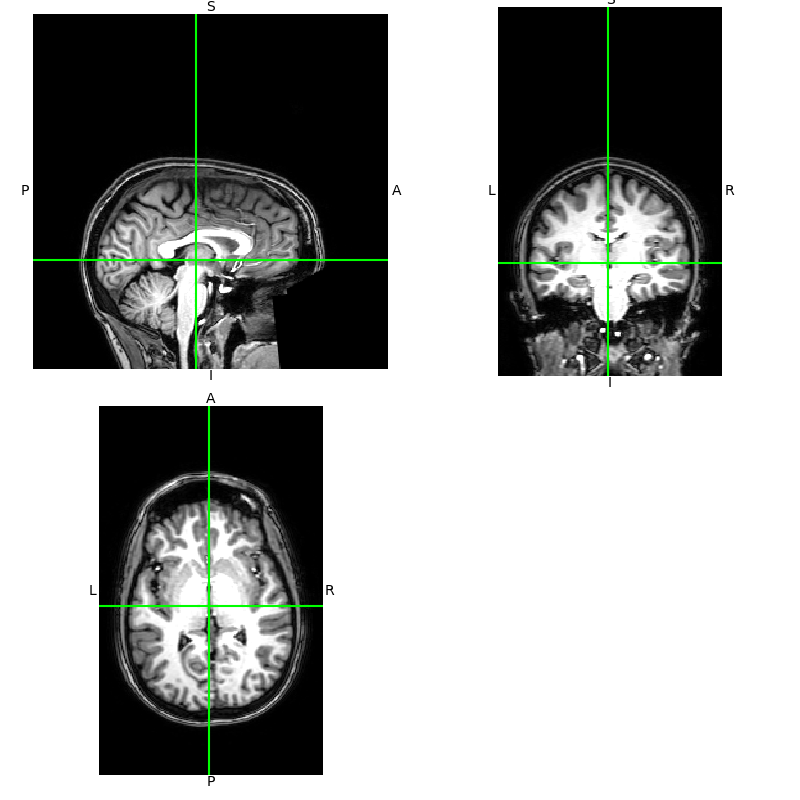
\includegraphics[width=\linewidth]{images/orthoview_t1w.png}
  \caption{T1w Modality High-Res 3d Scan of Subject Brain}
  \label{fig:ortho-t1w}
\end{figure}

\begin{figure}
  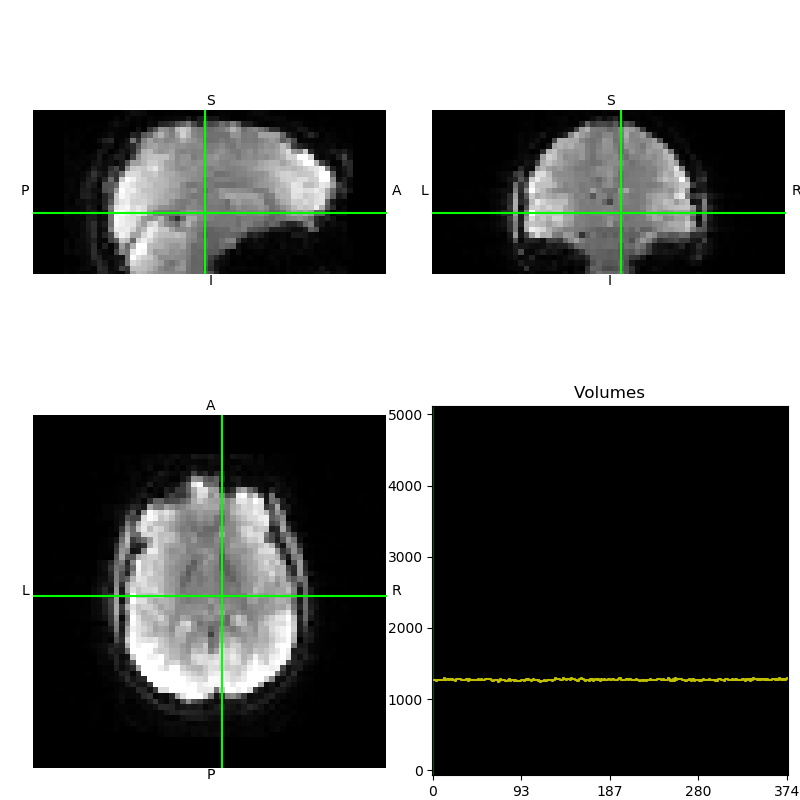
\includegraphics[width=\linewidth]{images/orthoview_bold.png}
  \caption{Bold Modality Low-Res 3d Experimental Scans of Subject Brain}
  \label{fig:ortho-bold}
\end{figure}

\begin{figure}
  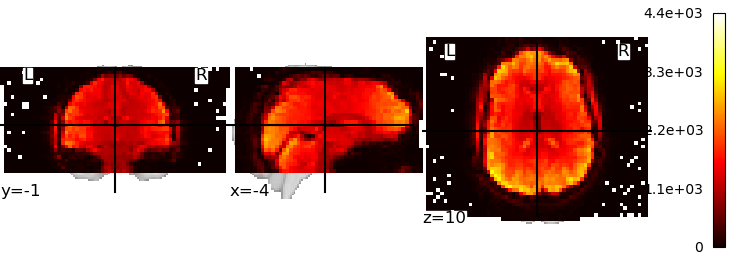
\includegraphics[width=\linewidth]{images/example_stat_map.png}
  \caption{Activity Measures from Bold Scans}
  \label{fig:ex_stat_map}
\end{figure}

\subsection{Review}\label{subsec:review}

You may review the full experimental paper as well here: \url{http://www.pamitc.org/documents/mermin.pdf}.

You may find this project repository here: (personal github link removed for anonymity)
Reading the paper is critical to understanding the format of the dataset, however I hope I will provide enough
abstraction in the project repository for you to be freed of that challenge should you wish to have a look around.

\section{Approach}\label{sec:approach}

Beginning with SKLearn~\cite{scikit-learn} data readiness was proven with moderately successful classification using
a simple SVM and then the SKLearn Multi-Layer-Perceptron neural network, getting 70-80\% accuracy, sufficing the
initial sanity check that deep learning would be ready to work on.

% TODO these are relevant citations, right?
Leveraging PyTorch~\cite{paszke2017automatic} first a framework for learning was likewise vetted using a simple fully
connected shallow network, graduating to the state of the art convolutional networks, chiefly focussed
on the ResNet~\cite{he2016deep} architecture styles, which have been developed for video classification~\cite{tran2018closer}
utilizing 3 dimensional convolutions much in the way 2 dimensional convolutions operate, which have
been shown to hold a slight edge on 2 dimensions~\cite{payan2015predicting} in other applications.


\subsection{Data Preparation}\label{subsec:data-preparation}

First as the data was not prepared for classification, critical cleaning include subtracting the mean image to better
highlight meaningful variance, and standardizing the data between 0 and 1.

Given the nature of the input images being 3d brain scans it's intuitive that examining the brain in 3 dimensions
allows for much more interesting patterns of brain activity and structuring being recognized.

This comes with a substantial cost however, as the extra dimension explodes the memory demands of the input data, and
the number of trainable parameters for the models.
Many of the recommendations following will vary based on the particular hardware, but with a 4GB GPU I had to be quite
careful about batch-sizes to not over-allocate memory.
To combat this, first, a relatively conservative amount of blank space is cropped from the images, halving the total footprint.
Following this, in order to use a batch-size of 64, I interpolate images to approximately $\frac{5}{6}$ their original dimension

In addition, I typically do not use the full cohort of 30 subjects, as I even encounter some RAM restrictions with the
full raw dataset consisting of
$64 sagital \times 64 coronal \times 30 axial \times 1 channel \times 32bit floats \times 375 scans \times 30 subjects$ or roughly 5.53 gigabytes

In working with 2 dimensions, omitting the axial dimension for a flat cross section, you'll see the dataset is
$\frac{1}{30}$ the size and hence, much more manageable.


\subsection{Examining the Data}\label{subsec:examining-data}

Two fully processed, correctly classified brain scans are presented in the figure~\ref{fig:comparison}
which pose a daunting challenge to human labelers.

\begin{figure}
  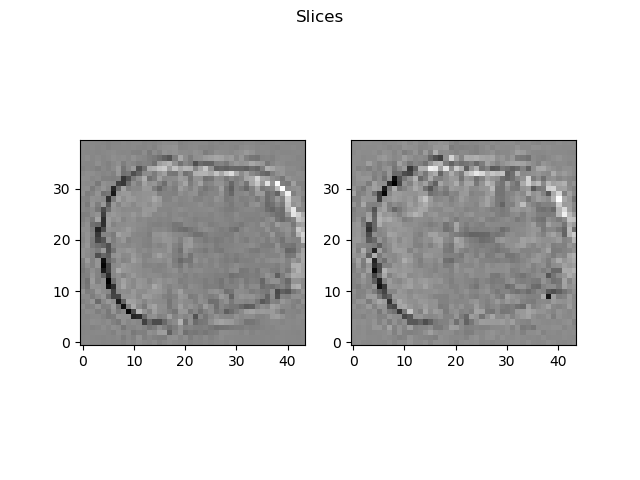
\includegraphics[width=\linewidth]{images/nf_f_hard_comparison.png}
  \caption{Nonfood-Stimuli \& Food-Stimuli Respectively from the same Subject}
  \label{fig:comparison}
\end{figure}

\subsection{Model Selection}\label{subsec:model-selection}

For the primary focus of comparing and improving classification accuracy using 2d and 3d architectures, ResNet models
of the standard 18 layers to 100+ layers are examined, as the ResNet family is both highly competitive, and demonstrated
in both 2 and 3 dimensions which will help comparisons in exploring the benefits of 3d brain scan usage.
Video processing typically limits the layers to a more shallow level than that of image processing, as unfortunately as
with the data, the model parameters explode out of control pretty fast, though some have seen minor improvements by
going deeper~\cite{hara3dcnns}.
The following parameter counts are from standard ResNet architectures adapted to a single input channel.

\begin{center}
 \begin{tabular}{||c c c||}
 \hline
 - & ResNet-18 2d & ResNet-18 3d \\ [0.5ex]
 \hline\hline
 Counts & 11,171,266 & 33,148,482 \\ [1ex]
 \hline
 Ratio & 1.0 & 2.97 \\ [1ex]
 \hline
\end{tabular}
\end{center}

\subsection{Comparisons}\label{subsec:comparisons}

Model performance is typically evaluated using accuracy, precision, recall, and AUC metrics, as well as total time to
train.

\section{Results}\label{sec:results}

With a complete experimental set-up, benchmark performance was established using the simple models ranging from the
SVM to the basic fully-connected network, at around 70-80\%.
Both 2 dimensional and 3 dimensional convolutional networks were able to surpass the benchmarks,
attaining 95\%+ accuracy.

The stretch goal of region highlighting using unsupervised segmentation proved infeasible for this project timeframe, given
the challenges overcome with the 3d convolutional model architecture.

\subsection{Model Architecture}\label{subsec:model-arch}

I explored the available hyperparameters of the chosen model architectures to a minor degree, focusing on
establishing optimal learning rates with the chosen optimizer and model, with the given normalized data.

Typically 1e-2 to 1e-4 worked, with learning rates on the order of 1e-3 being best for both ResNet style convolutional
networks.

Stochastic Gradient Descent with nesterov momentum on Cross Entropy Loss performed very well.
Other optimizers like Adam and loss metrics like NLL Loss explored were either on par or worse and thus not
further utilized.

None of my attempted customizations to the ResNet architecture netted any improvements, including expanding filter sizes
or adding normalization layers.

\subsection{Subject individuality}\label{subsec:subjects-individ}

Interestingly, performance of models on subjects not included in the training run was subpar.
For example, a model trained to 95\% accuracy on 6 subjects alone would fair closer to 60\% on 6 new subjects.
I speculate this is not overly worrisome, and a consequence of using such a small handful of subjects.
Better generalizability seems likely given an investment in much larger machinery or methodology capable of handling
more subjects, or better normalization practices.
One exploration of the data revealed by far most of the variance comes at the perimeter of the cortex suggesting slightly
varied sizes of brains not overlapping perfectly.
Convolutional networks should be able to tackle this dilemma with no problem but perhaps the small dataset makes
spatial and orientation noise more consequential.

\subsection{Training Progress}\label{subsec:training-prog}

Generally, training catches within about 20 epochs, learning to differentiate better than chance on 2
dimensional data~\ref{fig:2d_cold}, taking noticeably longer for 3 dimensional data~\ref{fig:3d_cold} to catch up,
as there's presumably more nuance to learn.
The learning rate may seem fairly aggressive~\ref{fig:cold_500_loss.png}
and takes one step back for every two steps forward, but overall produces
more competitive results than a gentler learning rate.

 \begin{figure}
  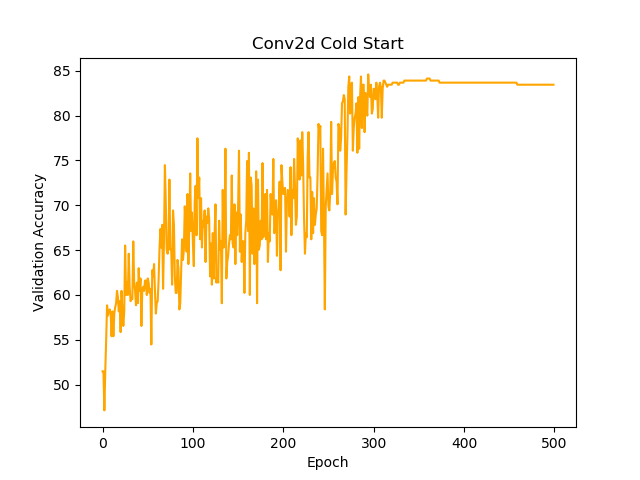
\includegraphics[width=\linewidth]{images/2d_cold.png}
  \caption{Cold-Start 2D Training Progress}
  \label{fig:2d_cold}
\end{figure}

 \begin{figure}
  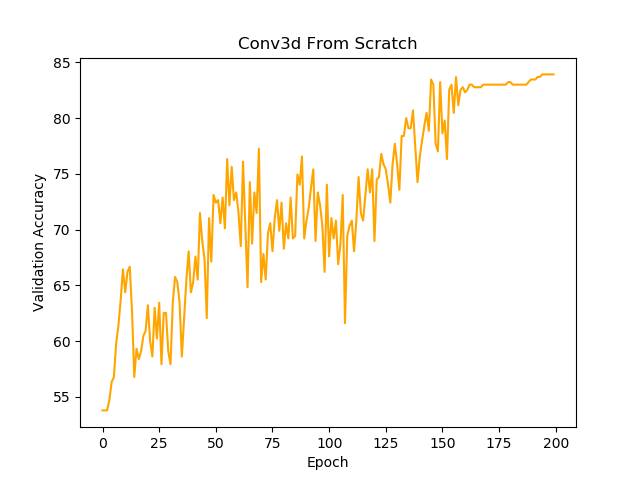
\includegraphics[width=\linewidth]{images/3d_cold.png}
  \caption{Cold-Start 3D Training Progress}
  \label{fig:3d_cold}
\end{figure}

 \begin{figure}
  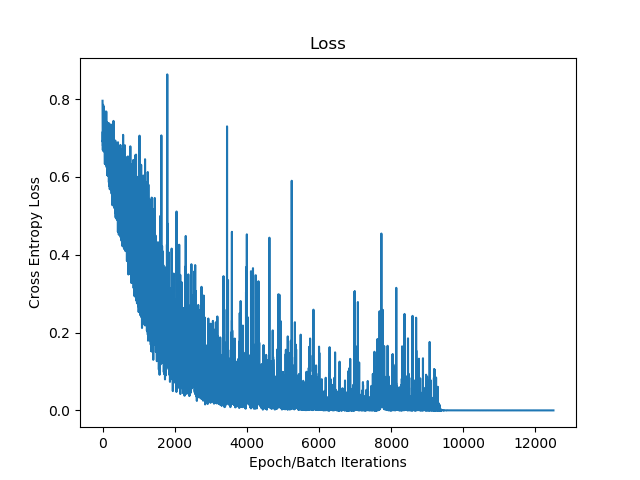
\includegraphics[width=\linewidth]{images/cold_500_loss.png}
  \caption{Cold-Start Training Progress Loss}
  \label{fig:cold_500_loss.png}
\end{figure}

\subsection{Warm Starts}\label{subsec:warm-starts}

Saving the model parameters and training again on a new subset of subjects or even resuming learning
on the same division worked wonderfully.

Getting the model to a stable, low 80\% performance leaves us in an excellent place to begin aggressively learning again.

With this method performances of over 95\%~\ref{fig:2d_warm} are common.

As mentioned before however, higher performances are typically seen on the same subject, though it doesn't take
long for the model to adapt to the new group of subjects for training, but of course it sacrifices performance on the
previous grouping to do so.

 \begin{figure}
  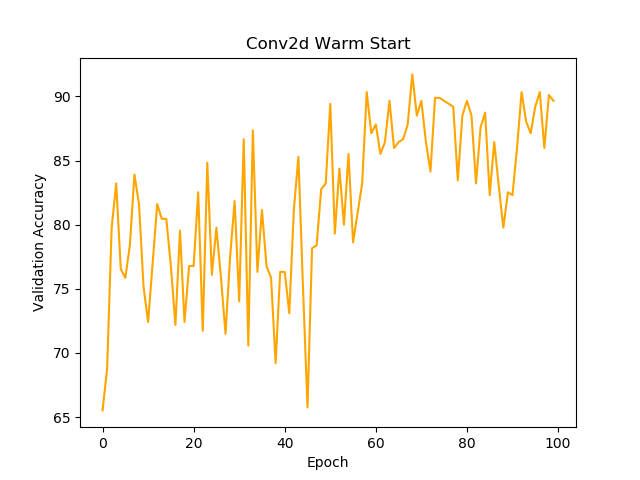
\includegraphics[width=\linewidth]{images/2d_warm.png}
  \caption{Warm-Start 2D Training Progress}
  \label{fig:2d_warm}
\end{figure}

\subsection{3 Dimensions}\label{subsec:3-dimensions}

One of the biggest challenges of this endeavor has been coping with the computational demands that the third
dimension adds.
Video data is notoriously large, and now I've seen 3d CNN's can be as well.
Our application here substitutes time for a third spatial axis, and does seem to be a richer dataset to draw from for
classification.
Training on a larger, more complex dataset does feel more challenging as well, with training taking longer to catch on
to something productive.

Unfortunately, I've found iterating with 3 dimensional models to be much harder than 2d which makes refinement also a
bit of a challenge.
Where training may take 15 minutes with a 2d CNN, it might be 5 hours or more with a 3d CNN, and the limitations on the
quality and abundance of the dataset size kick in much faster than for 2d.
The dataset is already a fairly conservative low-grade rendering of the brain and aggresive interpolation cuts into
performance directly.
Additionally, lowering the batch size is very detrimental to performance, with at least 64 images being critical to
learning generalizable patterns at each step in an epoch.
However, what I have seen in working with the 3d CNN's is that they are very performant, achieving on par or
3 to 4\% higher classification accuracy compared to their 2d counterparts, and responding encouragingly as well to warm-starts,
to which I'm very pleased.

\subsection{Performance Measures}\label{subsec:performance}

Here I examine one highly performant 2d convolutional network in more detail.
Thankfully it is a well balanced model, with seemingly high intuitive understanding of the differentiable characteristics
of brain activity, as it's highly accurate, and highly confident in it's decisions.

While I have been able to tweak the model to exceed this accuracy, this is in my opinion the most balanced
run observed as typically the model begins to favor performance on one class over the other despite near
equal representation.

 % P-R-F1-S
\begin{center}
 \begin{tabular}{||c c c||}
 \hline
 - & Nonfood & Food \\ [0.5ex]
 \hline\hline
Precision & 0.949074 & 0.958904 \\
 \hline
Recall & 0.957944 & 0.950226 \\
 \hline
F1 & 0.953488 & 0.954545 \\
 \hline
Support & 214 & 221 \\ [1ex]
 \hline
\end{tabular}

 % ROC-AUC / ACC
\end{center}
\begin{center}
 \begin{tabular}{||c c||}
 \hline
 ROC-AUC & Accuracy \\ [0.5ex]
 \hline\hline
  0.9847 & 0.954 \\ [1ex]
 \hline
\end{tabular}
\end{center}


\section{Discussion}\label{sec:discussion}

\subsection{Learning}\label{subsec:learning}
very cool! I tried spot checking different scans to see if I could tell the difference visually and I really really
cannot. I think it's encouraging that the model is able to notice impossible to visualize differences and run with it
this well. It's one thing to differentiate a st. bernard from a siamese cat, but two brain activations I'm not good at

\subsection{Future Works}\label{subsec:future-works}
Unsupervised segmentation, especially in 3d would be cool
Future works
- could strive to refine 3d more, with more time and compute
- unsupervised segmentation would be cool
- find ways to not have to smoosh images for memory?
- more visualizations? lack of color kinda sucks, saliency is weird, filters prob too

began work on visualization, it didn't lead anywhere useful, 1 channel might be a problem?
- check out filter viz
- see about unsupervised
- try 3d alternative archs? (dont really need to)

might want to improve 3d before going on to segmentation,
- scheduler / hyperparams / diff architectures (just go with res3d, res2d+1d, mix three types
wowee good stuff, hope to use a LR scheduler in the future to try to control this better?


 I'd be stoked
to reproduce on 3d, and trusting the model this much, open the door to segmentation

model ensemble (free extra few percent perf)
 \begin{figure}
  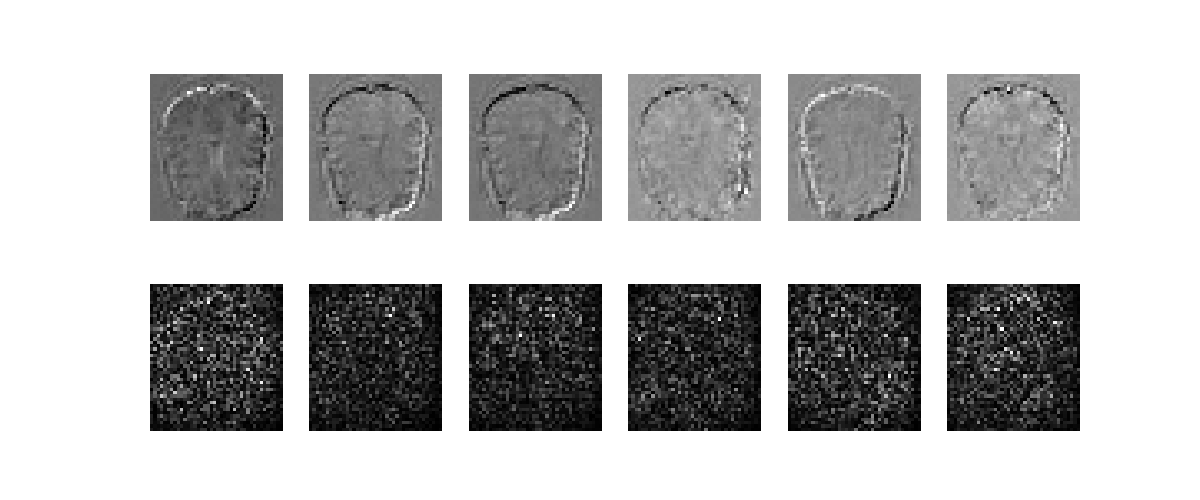
\includegraphics[width=\linewidth]{images/saliency.png}
  \caption{caption}
  \label{fig:saliency}
\end{figure}


% ----------------------------------------------------------------------
% END
% ----------------------------------------------------------------------
{\small
\bibliographystyle{ieee}
\bibliography{project}
}

% ----------------------------------------------------------------------
% SUPPLEMENTARY
% ----------------------------------------------------------------------
\section{Supplementary Material}\label{sec:supplementary}

Extra material for reference



 \begin{figure}
  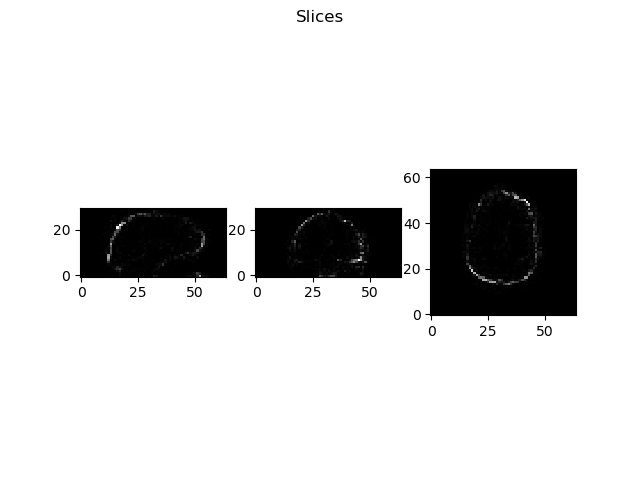
\includegraphics[width=\linewidth]{images/var_on_cortex_2.png}
  \caption{caption}
  \label{fig:cortex-var}
\end{figure}

\end{document}

